Extensive experiments have been done to validate our design of VTC as well as evaluate 
its performance under various scenarios. This section covers our testbeds, experiment 
methodologies, performance tuning, results, and analysis. 

\subsection{Experiment setup}
The experiments are conducted in two phases. In the first phase, only CPU is over-committed 
to validate the design of VTC with over-commitment. In this phase, we used a cluster of 18 nodes (1 login node, 1 management node, and 16 compute nodes) to mimic a realistic HPC computing environment. Each node has dual 10-core Intel Xeon E5-2660 processor and 128 GB DDR4 memory. %, and 10 Gb Ethernet. 
The hypervisor used is VMware ESXi 6.5, OS is CentOS 7.3, and resource manager is TORQUE 6.1 with the default job scheduler. We use compute-intensive benchmarks from PolyBench/C 3.1 and BioPerf~\cite{1526013}. 
In the second phase, we evaluate the full-fledged VTC design with both CPU and memory over-commitment on another testbed with huge memory capacity for memory-intensive workloads. The second cluster has 1 login, 1 management, and 8 compute nodes. Each node has dual 16-core Intel Xeon Gold 6130 processor and 768 GB memory. %, and 10 Gb Ethernet. 
The hypervisor used is VMware ESXi 6.7, OS is CentOS 7.6, and resource manager is TORQUE 6.1 with the default job scheduler. We add memory-intensive benchmarks from HPCC~\cite{dongarra2004introduction}.

\subsection{CPU over-commitment}
For performance evaluation, each node is installed with two execution environments on two separate booting disks, that is, a native OS and an ESXi hypervisor. With the hypervisor, we further define three VTC scenarios: 1) one virtual cluster; 2) two virtual clusters; 3) four virtual clusters. The latter two scenarios have 2X and 4X CPU over-commitment, respectively. 
When comparing performance among different execution scenarios (including bare metal cluster), we run the same job stream which consists of 3248 jobs that are randomly sampled from the PolyBench and BioPerf suites, and the wall clock execution time is shown in Figure~\ref{fig:cpu_exe_time}.

\begin{figure}[!t]
   \begin{center}
       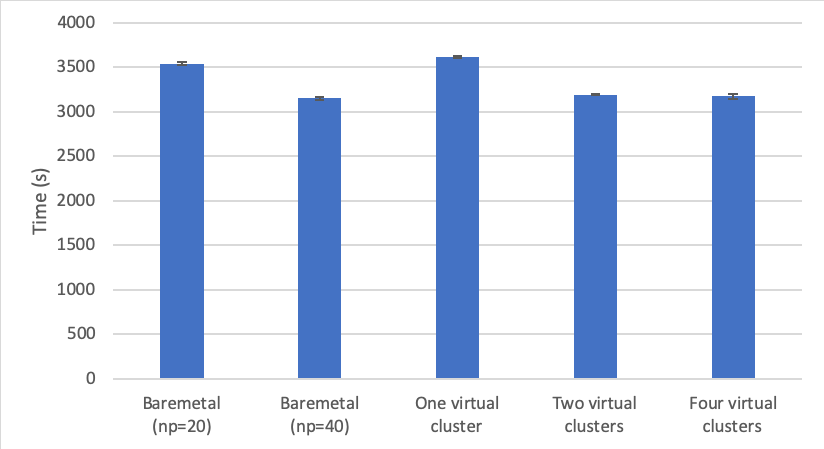
\includegraphics[width=\columnwidth]{Figures/cpu_exe_time}
   \end{center}
   \caption{Comparison of wall clock execution time for a job stream between bare metal and VTC with different CPU over-commitment ratios. Results are average of three runs.}
   \label{fig:cpu_exe_time}
 \end{figure}

Because each node in our testbed has 20 cores, in the first experiment we configured each TORQUE worker with 20 job slots. As reflected in Figure~\ref{fig:cpu_exe_time}, the execution with one virtual cluster is very close to that of bare metal (first column), with only a 2.2 percent overhead. Furthermore, when multiple virtual clusters are used with CPU over-commitment, the execution time is surprisingly shorter, implying an improved throughput despite the virtualization overhead. Through careful analysis, we identified that the throughput improvement can mainly be attributed to increased CPU utilization when more jobs are concurrently scheduled to execute. This has been verified by modifying each TORQUE worker in the bare-metal environment to use 40 job slots, after which the throughput is improved to the same level as the over-committed virtual environment. This can be seen in the second column of Figure~\ref{fig:cpu_exe_time}.

Besides execution time, another performance metric that we monitored is the total CPU utilization across the whole cluster. On the ESXi hypervisor, we used esxtop running on each compute node to sample CPU utilization of all VMs at 5-second intervals, and the results for one, two, and four virtual clusters are shown in Figure~\ref{fig:cpu_utilizations}. With two and four virtual clusters, the decreasing trend at the end is due to job completion. Clearly, CPU utilization is consistent with the job execution times in Figure~\ref{fig:cpu_exe_time}. For example, the lowest CPU utilization case--one virtual cluster--matches the longest job execution time. The higher CPU utilization with two and four virtual clusters is due to resource consolidation brought about by virtualization. That is, when multiple virtual clusters share a physical cluster, the CPU scheduler on each ESXi host has more jobs to schedule and is therefore able to make better scheduling decisions by taking advantage of Hyper-Threading and eliminating idle cycles. At the same time, improved utilization comes with better consistency, where the utilization with two and four virtual clusters is much smoother than in the single-cluster case.

\begin{figure}[!t]
   \begin{center}
       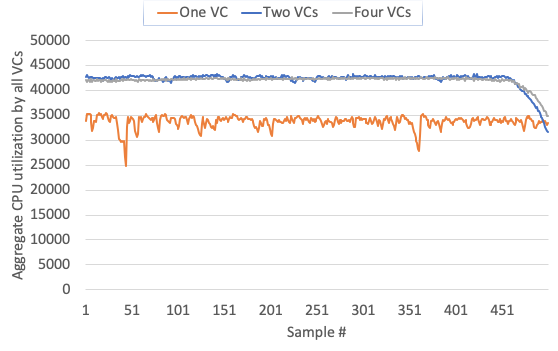
\includegraphics[width=\columnwidth]{Figures/cpu_utilizations}
   \end{center}
   \caption{Aggregate CPU utilization across 16 nodes at 5-seconds intervals.}
   \label{fig:cpu_utilizations}
   \vspace{-0.2in}
 \end{figure}

 In a production cloud environment, an important principle is fairness when multiple tenants are sharing the computing resources. We further examined the per-cluster CPU utilization in the multiple-cluster cases, and the case of four virtual clusters is shown in Figure~\ref{fig:per_cluster_utilization}. It is clear that the ESXi scheduler effectively maintains fairness so that each virtual cluster gets the same amount of CPU resources. The case of two virtual clusters is 
 the same thus not discussed. 


\begin{figure}[!t]
   \begin{center}
       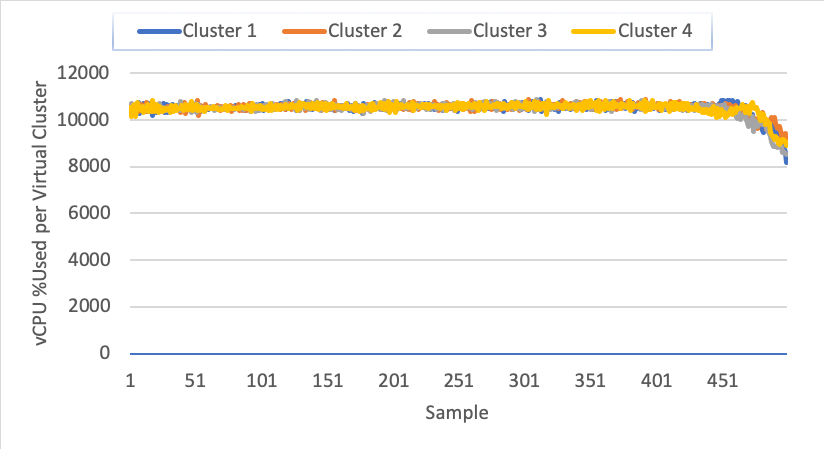
\includegraphics[width=\columnwidth]{Figures/per_cluster_utilization}
   \end{center}
   \caption{Plot of CPU utilization per virtual cluster at 5-seconds intervals for fairness check.}
   \label{fig:per_cluster_utilization}
   \vspace{-0.2in}
 \end{figure}

\subsection{CPU over-commitment with shares}
In addition to the option of equally sharing resources, the proportional, share-based scheduler of the ESXi hypervisor offers a very useful degree of flexibility. This subsection continues the CPU over-commitment study by configuring virtual clusters with different shares, to demonstrate the capability of creating a multi-tenant environment with quality-of-service guarantees. 

With the use of CPU shares, each VM can be given a particular guaranteed share of CPU resources. When there are multiple VMs running on an ESXi host, the ESXi scheduler allocates CPU based on the ratio of shares among all the running VMs. This feature extends to a virtualized HPC cloud. Specifically, each user or group can be given an appropriate share of the physical system when their virtual cluster is allocated. In this experiment, we focus on the case of four virtual clusters and set the shares ratio among the four VMs as 2:1:1:1 on every compute node. The CPU utilization is shown in Figure~\ref{fig:share_utilization}. Clearly, the CPU utilization ratio among the virtual clusters is the same as the specified shares ratio. Another important observation is that the aggregate CPU utilization across 4 virtual clusters is the same as previous no-shares case as depicted in Figure~\ref{fig:cpu_utilizations}.


\begin{figure}[!t]
   \begin{center}
       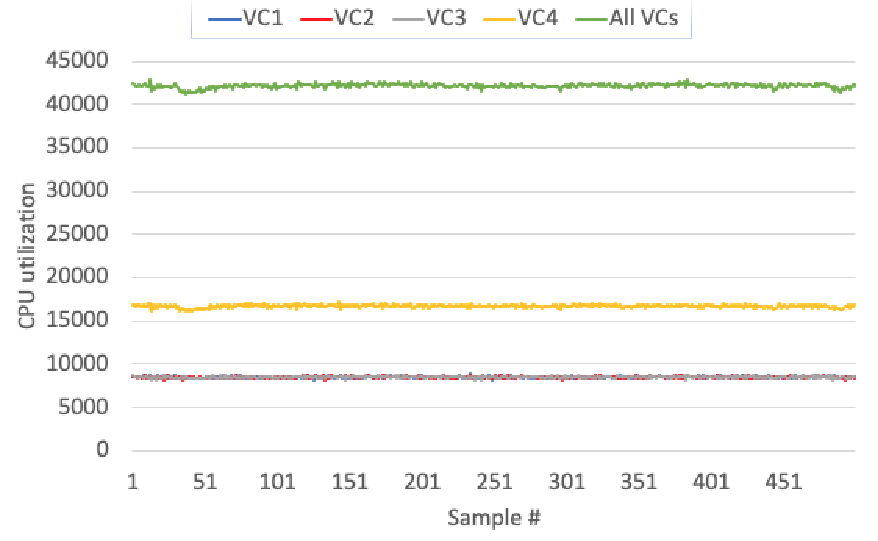
\includegraphics[width=\columnwidth]{Figures/share_utilization}
   \end{center}
   \caption{CPU utilization for four virtual clusters with 2:1:1:1 CPU shares. Utilization is sampled at 5-second intervals.}
   \label{fig:share_utilization}
 \end{figure}

\subsection{CPU + memory over-commitment}
Given that memory over-commitment is more challenging, we only test two virtual clusters with 2X CPU and memory over-commitment. vSphere Dynamic Resource Scheduler (DRS) is used to dynamically control VM migration for load balancing~\cite{infrastructure2006resource}. Considering the VM migration cost, we decided to use four quarter-size VMs to replace the single full-size VM on each node for each tenant. As a result, each tenant in this experiment gets a virtual cluster of 32 VMs across the 8 node cluster. 

To stress the system memory, we added benchmarks from HPCC. For all these HPCC benchmarks, a problem size of 53664 is chosen to have the memory consumption ranging from 16 GB to 22 GB per job instance. All the benchmarks are run with a single threaded process to mimic throughput workloads. 
To model a real HPC tenant, we specify the job arrival time to follow a Gamma distribution based on the study of several production HPC systems~\cite{lublin2003workload}.  
The resulted mean job inter-arrival time is 20.88 seconds
%The Gamma distribution has a shape parameter of 10.23 and scale parameter of 0.49. With those parameters, the mean job inter-arrival time is 10.23 / 0.49 = 20.88 seconds. 
%Also, all job sequences are shuffled to generate randomized job streams. Then, two execution scenarios are designed to represent different workload patterns. 

Two execution scenarios are designed to represent different workload patterns. In the first scenario, 1600 HPCC jobs (memory-intensive) are submitted to the first virtual cluster all at the beginning, while 1500 BioPerf jobs (memory-light) arrive at the second virtual cluster following the above Gamma distribution. The number of jobs are determined to let the two virtual clusters finish at roughly the same time. In the first virtual cluster, all the job slots will be consumed immediately and the jobs will maximize their utilization of the cluster's CPU and memory resources. In the second cluster, CPU and memory load will gradually build up. 
We make the second scenario more demanding by running two HPCC streams of 1600 jobs following the Gamma distribution. 
%Were all job slots being used, the active memory consumption would largely exceed the physical memory capacity. 
It's demanding because, even if each job only consumes 16 GB memory, 64 job instances on each node will require 64 * 16 GB = 1024 GB, which is much larger than the node capacity. It is well understood that ESXi cannot support that kind of memory over-usage. But, it is still worthwhile to explore in the realistic case where jobs randomly come and go, whether DRS can collaborate with ESXi memory reclamation techniques to accommodate this usage pattern. 

In each scenario, we run w/ and w/o DRS and measure two metrics: 1) wall clock time (WCT), i.e., the elapsed time from the start of job submission to the completion of the last job; 2) cumulative job execution time (CJET), i.e., the cumulative sum of all job instances' execution time. 

%The first metric is a measure of the system throughput, and the second metric indicates system efficiency. 
The results in scenario 1 are plotted in Figure~\ref{fig:memory_scenario1}. As the figures suggest, while VTC successfully supported 2X CPU and memory over-commitment regardless of DRS, DRS reduces HPCC's WCT by 11.1\%, which is a great improvement in throughput. 
The reason why DRS doesn't reduce BioPerf's WCT is that BioPerf jobs strictly follow the Gamma distribution in job arrivals.
But as we can see in Figure~\ref{fig:memory_cjet}, DRS reduces BioPerf's CJET by 18.4\%, making room available for more jobs. HPCC's CJET slightly increases with DRS and it indicates that DRS can cause minimal overhead to individual jobs due to telemetry sampling and VM migration. 
%, but increases HPCC CJET by 1.1\%, which is negligible. 
The number of VM migrations in each run is in the range of 30-40. It's interesting to notice that all migrations happened to the BioPerf VMs, which is because BioPerf VMs have smaller memory footprint and are lighter to migrate.

\begin{figure}
     \centering
     \begin{subfigure}[b]{0.45\textwidth}
         \centering
         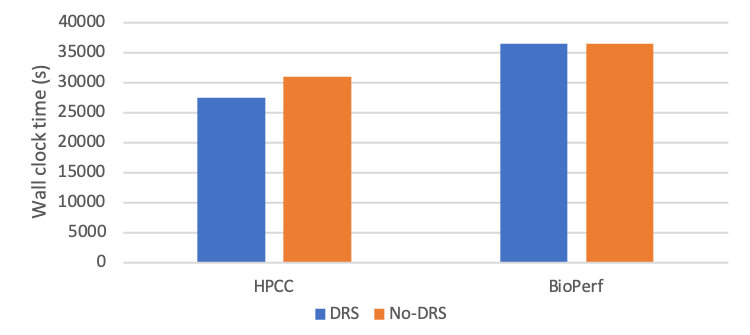
\includegraphics[width=\textwidth]{Figures/memory_wct}
         \caption{Wall clock time}
         \label{fig:memory_wct}
     \end{subfigure}
     \hfill
     \begin{subfigure}[b]{0.45\textwidth}
         \centering
         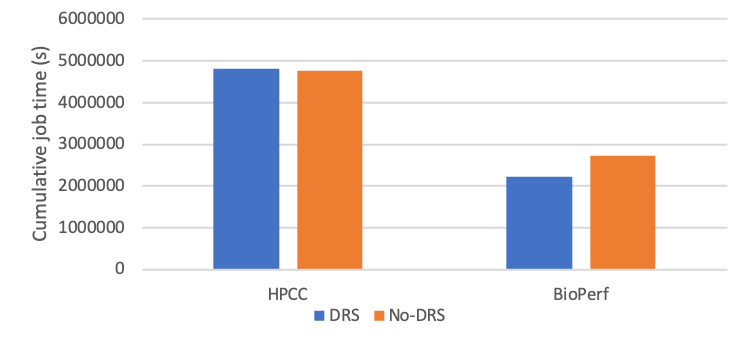
\includegraphics[width=\textwidth]{Figures/memory_cjet}
         \caption{Cumulative job execution time}
         \label{fig:memory_cjet}
     \end{subfigure}
     \caption{Comparison between DRS enabled and DRS disabled for VTC with 2X CPU and memory over-commitment. Workloads are from scenario 1. }
     \label{fig:memory_scenario1}
\end{figure}

As mentioned above, the second scenario is much more demanding because HPCC jobs can potentially consume all the configured VM memory. It's not a surprise the cluster is not able to finish two simultaneous streams of HPCC jobs, regardless of whether DRS is used. The guest OS encountered CPU soft lockup errors when hypervisor swapping occurs and when swapping is not responsive enough. Our analysis identified HPL (one benchmark in the HPCC suite) jobs as the bottleneck. Each HPL job needs more than 3 hours to finish, and once enough HPL instances accumulate on any node, the hypervisor is not able to handle their excessive memory requirements. Therefore, we decided to remove HPL from the job stream. After this change, we see that two HPCC streams can finish when DRS is on. Without DRS, the same failure occurs. Clearly, this demonstrates the effectiveness of DRS in load balancing and mitigating memory pressure. 

Though HPCC VMs are heavier to migrate, on average 67 VM migrations occurred per run, due to the extreme memory stress. Naturally, one may concern that the large number of migrations could introduce jitters to the running workloads. To quantify that, we collect the execution time distribution among all instances for each benchmark. It turns out that the execution time is quite consistent. For example, the histogram for RandomAccess (another benchmark in the HPCC suite) is shown in Figure~\ref{fig:ra_histogram}.

\begin{figure}[!t]
   \begin{center}
       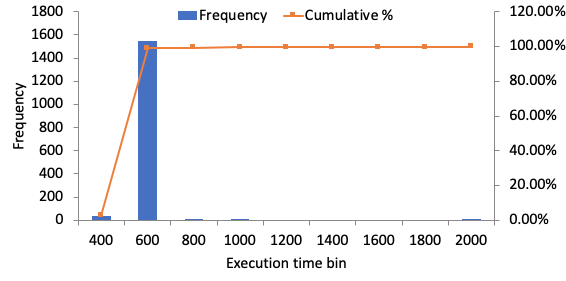
\includegraphics[width=\columnwidth]{Figures/ra_histogram}
   \end{center}
   \caption{Histogram of individual RandomAccess job execution time from both virtual clusters.}
   \label{fig:ra_histogram}
 \end{figure}




